\chapter*{Costs and benefits of test automation}

We get more benefit from testing the riskier parts of our application - whether that's technical risk or business risk. We've also got to consider how easy it is to automate each part of the application.

Each of the four statements below fits into a different section of the quadrant - can you decide which goes where?

\begin{itemize}
    \item Always try to automate
    \item May be worth automating
    \item Pointless to invest in automation
    \item Invest in specialised automation framework or tool
\end{itemize}

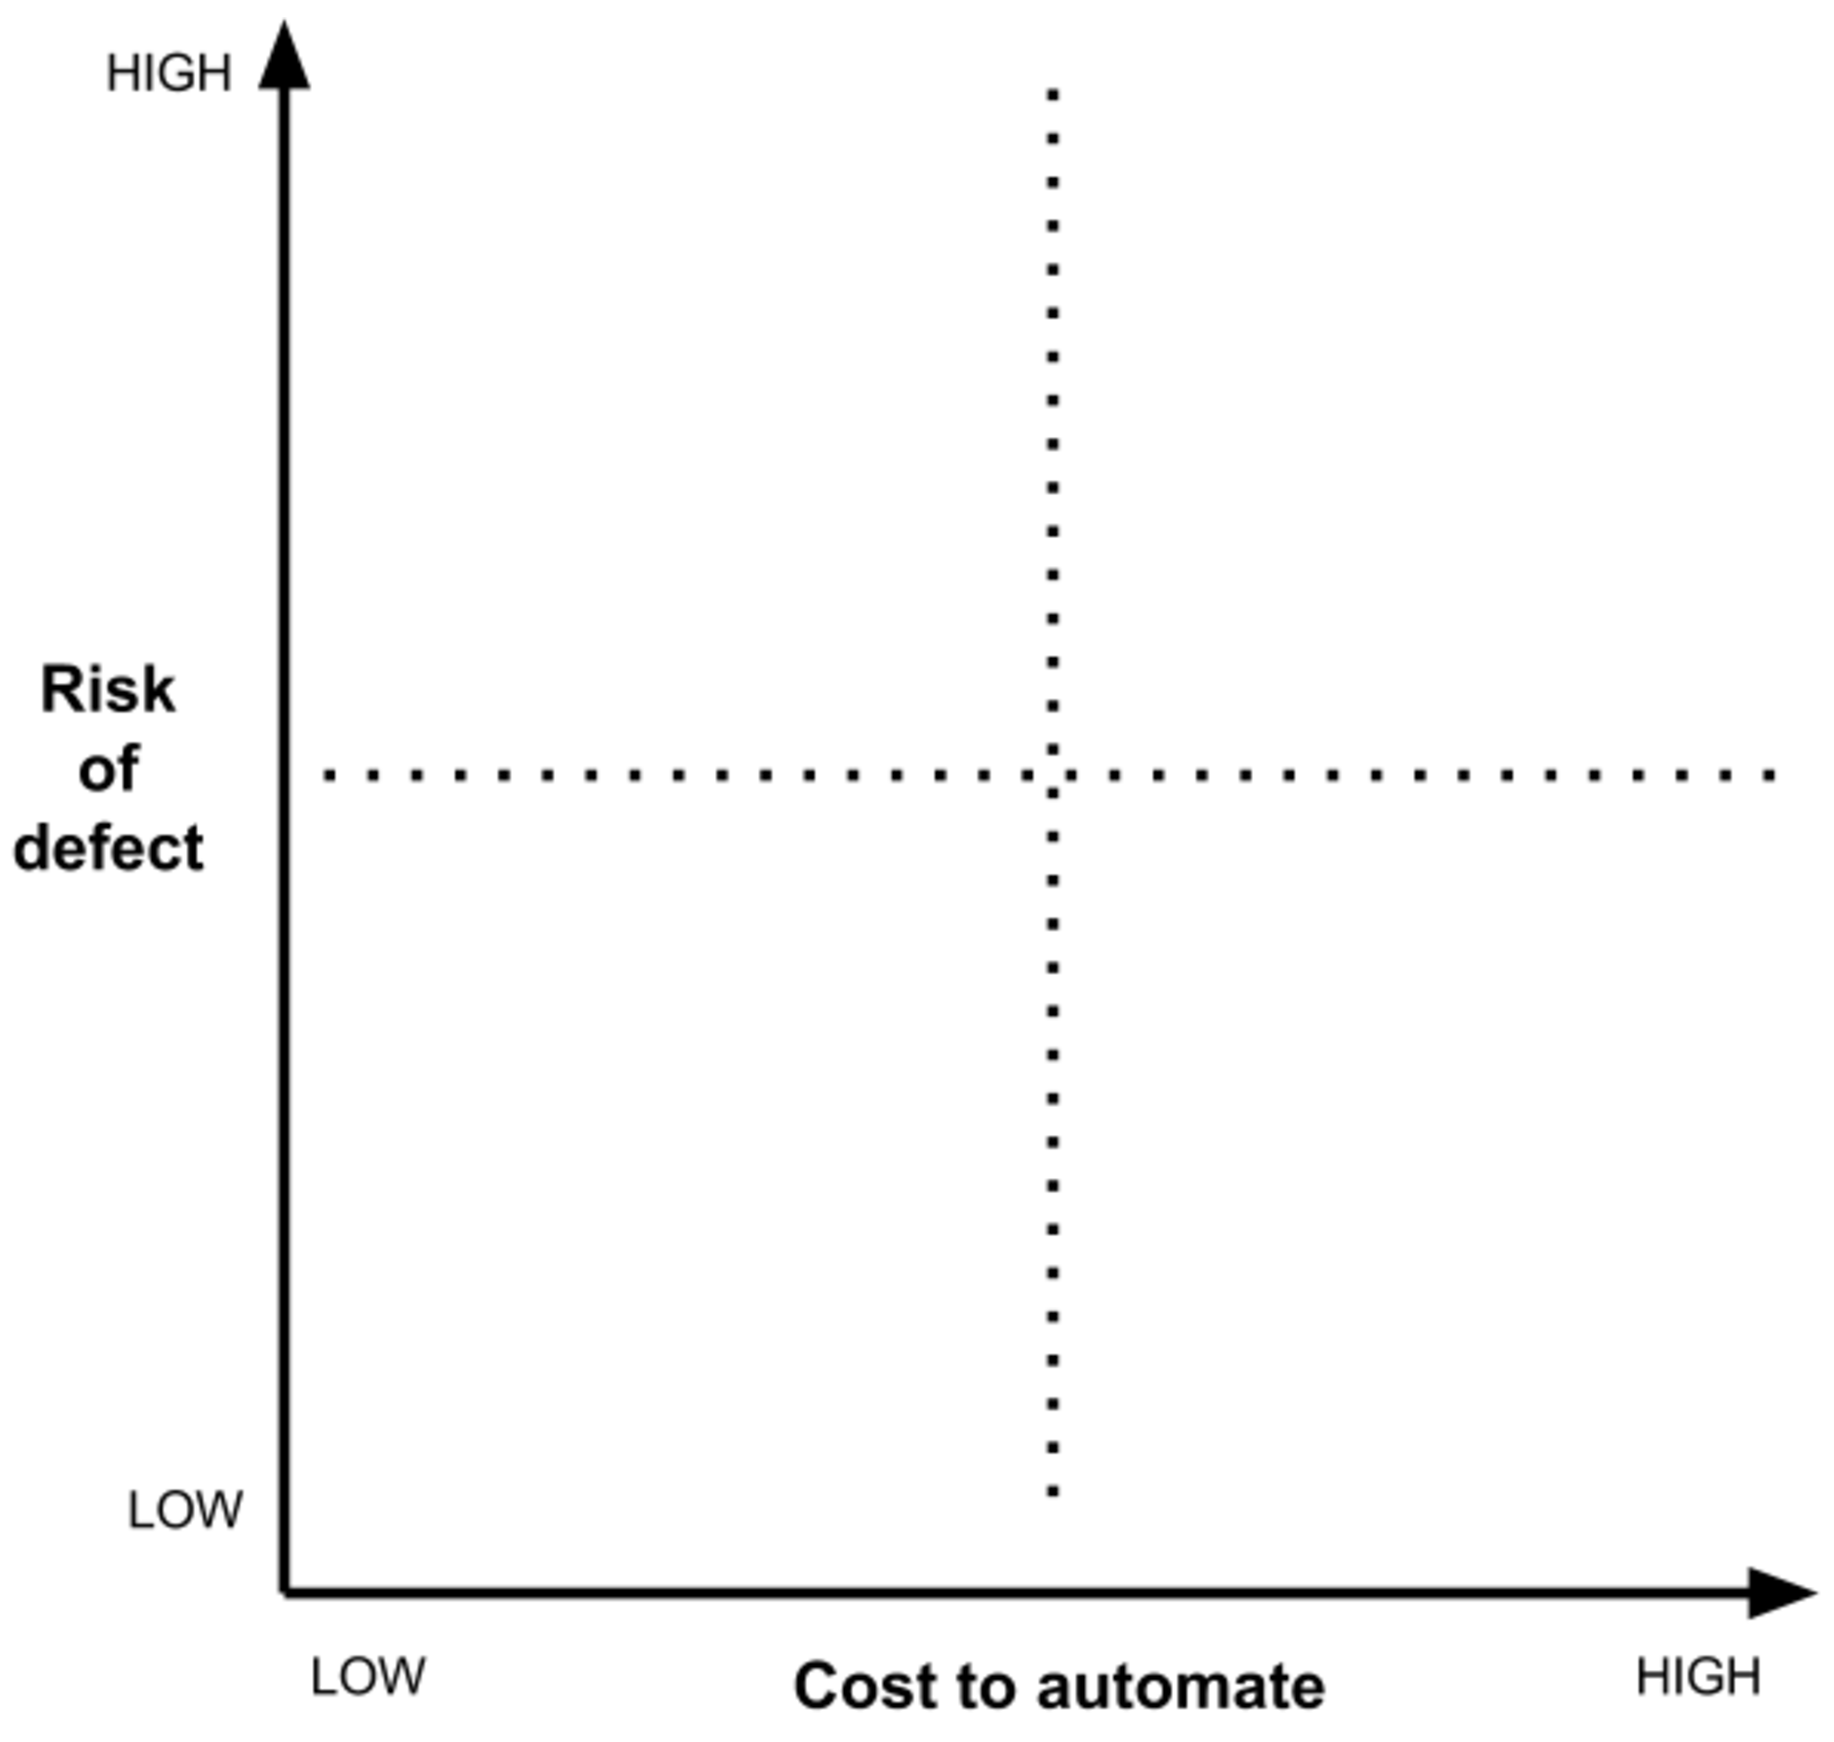
\includegraphics[width=\textwidth]{images/risk-benefit-quadrant}


\section*{Think about testing your work}

Are there some types of defects that you encounter regularly?

\answerbox{4}

Manual testing often consists of repetitive, scripted activities. What prevents you from automating those parts?

\answerbox{4}

Does your product depend on external services, systems or libraries? Could 'stubbing' out any of these dependencies make testing easier? What risks might 'stubbing' cause?

\answerbox{4}

Where in the quadrant above does your work typically fit? Why?

\answerbox{4}
